\documentclass[11pt,a4paper]{article}

\usepackage[utf8]{inputenc}
\usepackage[T1]{fontenc}
\usepackage[spanish,es-nodecimaldot,es-noshorthands]{babel}
\usepackage[margin=2cm]{geometry}
\usepackage{lmodern}
\usepackage{microtype}
\usepackage{enumitem}
\usepackage{booktabs}
\usepackage{graphicx}
\usepackage{tikz}
\usetikzlibrary{positioning,arrows.meta,calc}
\usepackage[hidelinks]{hyperref}
\usepackage{titlesec}

\titlespacing*{\section}{0pt}{8pt}{3pt}
\setlist{nosep, leftmargin=*}
\setlength{\parskip}{3pt}
\setlength{\parindent}{0pt}
\setlength{\textfloatsep}{8pt}
\setlength{\floatsep}{6pt}
\setlength{\intextsep}{6pt}

\title{\vspace{-1.2cm}\textbf{Detección de exoplanetas en curvas de luz de Kepler:\\
features físicas versus redes convolucionales 1D}\\[2pt]
\large INF396 -- Informe de avance}
\author{Noelia Morales \quad Matías Lara\\
\small Ingeniería Civil Informática, Universidad Técnica Federico Santa María}
\date{\vspace{-0.6cm}}

\begin{document}
\maketitle

% ------------------------------------------------------------------
\section{Problema y objetivo}

Una curva de luz es la medición del brillo de una estrella a lo largo del
tiempo, registrada por el telescopio espacial Kepler. Cuando un planeta pasa por
delante de su estrella, bloquea una pequeña fracción de su luz y el brillo baja
durante unas horas (un \emph{tránsito}); como el planeta orbita, la caída se
repite con regularidad. Es como observar un faro lejano: si cada cierto tiempo
algo pasa por delante y lo apaga brevemente, deducimos que algo gira a su
alrededor.

Detectar esa señal es difícil: la caída es diminuta, del orden de 0{,}01\% a
1\% del brillo, y comparable al ruido. Además, las estrellas varían su brillo
por sí solas (manchas, rotación, erupciones) y el telescopio introduce errores
de medición. A esto se suma que las estrellas con planeta confirmado son
extremadamente escasas: 37 de 5.087 en el entrenamiento (0{,}73\%). Un modelo
que prediga siempre ``sin planeta'' obtiene 99{,}27\% de \emph{accuracy} sin
detectar ninguno, por lo que esta métrica no sirve en este problema.

En la literatura, las redes convolucionales han mostrado ser efectivas para
clasificar señales de tránsito en datos de Kepler~\cite{shallue2018,ansdell2018},
y los clasificadores de \emph{gradient boosting} sobre features extraídas de la
curva alcanzan resultados comparables con un costo computacional mucho
menor~\cite{malik2022}. Sobre el mismo dataset que usamos, Priyadarshini y
Puri~\cite{priyadarshini2021} reportan 99{,}62\% de \emph{accuracy} con un
ensamble de CNN, cifra poco informativa dado que un clasificador trivial obtiene
99{,}12\% en el mismo conjunto de prueba.

\textbf{Objetivo.} Comparar un clasificador basado en features con significado
físico contra una red neuronal convolucional 1D para detectar exoplanetas en
curvas de luz de Kepler, con un protocolo de evaluación adecuado al fuerte
desbalance de clases, y analizar mediante técnicas de interpretabilidad qué
patrones aprende la red. En concreto: (1)~baseline con features físicas (FFT y
periodograma BLS) y modelos Random Forest y XGBoost; (2)~CNN 1D sobre la curva
preprocesada; (3)~estudio de ablación; (4)~interpretabilidad con mapas de
saliencia y Grad-CAM 1D~\cite{selvaraju2017}.

\textbf{Ajustes respecto a la propuesta.}
\begin{itemize}
  \item \emph{PR-AUC} es la métrica principal; el conjunto de prueba oficial
  (solo 5 positivos) se usa como confirmación y no para decidir.
  \item La CNN se evaluó con 5 folds $\times$ 1 repetición (el baseline con
  5 $\times$ 5) por costo de cómputo.
  \item La CNN de esta etapa aún no usa \emph{data augmentation} ni ajuste de
  hiperparámetros: se reporta como versión inicial.
  \item Se agregó al preprocesamiento un recorte de picos hacia arriba, que no
  figuraba en la propuesta (ver Sección~\ref{sec:datos}).
\end{itemize}

% ------------------------------------------------------------------
\section{Solución propuesta}

La Figura~\ref{fig:pipeline} resume el enfoque: una misma curva preprocesada
alimenta dos ramas que se comparan bajo el mismo protocolo de evaluación.

\begin{figure}[h]
\centering
\begin{tikzpicture}[
  box/.style={draw, rounded corners, align=center, font=\footnotesize, inner sep=3pt, minimum height=0.9cm},
  pend/.style={box, dashed},
  >=Stealth, node distance=0.5cm and 0.45cm]
  \node[box] (data) at (0,0) {Curvas\\crudas\\(3.197 pts)};
  \node[box] (pre) at (2.7,0) {Preprocesamiento\\detrending $\to$ recorte\\$\to$ normalización};
  \node[box] (feat) at (5.9,0.95) {Features:\\estadísticos,\\FFT, BLS};
  \node[box] (rf) at (8.3,0.95) {Random Forest\\XGBoost};
  \node[box] (cnn) at (8.3,-0.95) {CNN 1D\\(curva completa)};
  \node[box] (ev) at (11.0,0) {Evaluación\\CV 5$\times$5 +\\bootstrap};
  \node[pend] (ab) at (14.2,0) {Ablación e\\interpretabilidad\\(pendiente)};
  \draw[->] (data) -- (pre);
  \draw[->] (pre.east) -| (feat.south);
  \draw[->] (pre.east) -| (cnn.west);
  \draw[->] (feat) -- (rf);
  \draw[->] (rf.east) -| (ev.north);
  \draw[->] (cnn.east) -| (ev.south);
  \draw[->] (ev) -- (ab);
\end{tikzpicture}
\caption{Esquema general de la solución. Las cajas punteadas están pendientes.}
\label{fig:pipeline}
\end{figure}

\textbf{Rama A: features físicas.} Se extraen 18 features por estrella:
8~estadísticos de la distribución del flujo (mínimo, percentiles 1 y 5,
desviación, asimetría, curtosis, y conteo de puntos bajo $-3\sigma$ y $-5\sigma$);
4~del espectro de Fourier (frecuencia y relevancia del pico dominante, fracción
de potencia en bajas y altas frecuencias); y 6~del periodograma \emph{Box Least
Squares} (BLS)~\cite{kovacs2002}. El BLS busca una caída rectangular repetida:
para cada par (período, duración) pliega la curva y mide qué tan bien se alinean
las caídas. Se exploran 3.000 períodos entre 0{,}5 y 30 días y 4 duraciones
(0{,}05 a 0{,}3 días); de la mejor ``caja'' se toman período, duración,
profundidad, SNR, contraste frente al periodograma típico y número de tránsitos
que caben en la curva. Sobre estas features se entrenan Random Forest (300
árboles, \texttt{balanced\_subsample}) y XGBoost (300 árboles, profundidad~3,
\texttt{scale\_pos\_weight} = negativos/positivos del fold de entrenamiento).

\textbf{Rama B: CNN 1D.} Recibe la curva preprocesada (recortada a $[-30,5]$) y
aprende sus propios patrones: tres bloques Conv1D (16, 32 y 64 filtros, núcleos
de 7, 5 y 5) con BatchNorm, ReLU y MaxPool, un \emph{global max pooling} que
responde ``¿algún filtro encontró su patrón en alguna parte de la curva?'', un
\emph{dropout} de 0{,}3 y una capa lineal. Se entrena con entropía cruzada
ponderada (\texttt{pos\_weight} = negativos/positivos), Adam (tasa 10$^{-3}$),
20 épocas fijas y lotes de 64. No se usa parada temprana: con unos 7 positivos
por fold, un conjunto de validación interno sería demasiado ruidoso.

\textbf{Evaluación.} Validación cruzada estratificada de 5 folds repetida
5 veces sobre el entrenamiento (1 vez para la CNN), con recall, precisión, F1 y
PR-AUC; intervalos de confianza al 95\% por \emph{bootstrap} estratificado
(1.000 remuestras) en el conjunto de prueba. Las features y el preprocesamiento
se calculan estrella por estrella, por lo que no hay fuga de información entre
folds.

\begin{figure}[h]
\centering
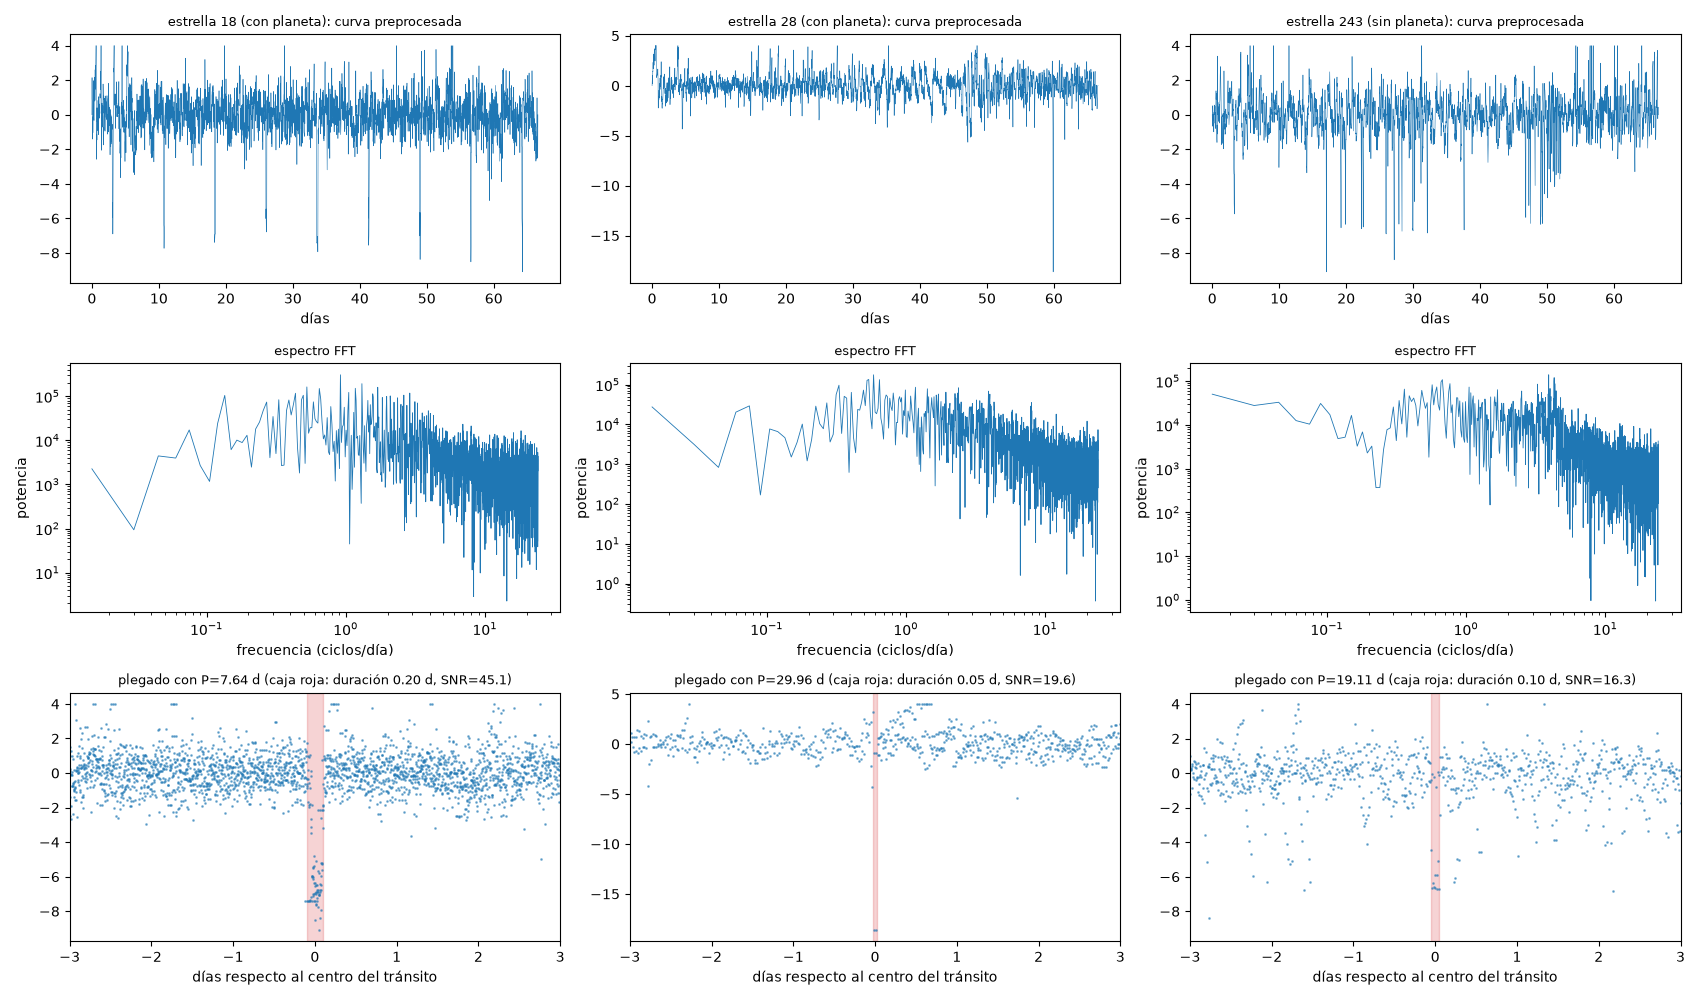
\includegraphics[width=0.88\textwidth]{../../results/04_fft_bls_ejemplo.png}
\caption{Curva preprocesada, espectro FFT y plegado BLS de tres estrellas. En
la estrella 18 (con planeta) el plegado con $P=7{,}64$ d apila caídas de unos
$-7\sigma$ (SNR 45); en la 28 (con planeta) el BLS se apoya en una sola caída
profunda; en la 243 (sin planeta) las caídas no se alinean. La FFT no muestra un
pico claro en ninguna.}
\label{fig:bls}
\end{figure}

% ------------------------------------------------------------------
\section{Plan de implementación}

El código está en un repositorio de GitHub con lógica reutilizable en
\texttt{src/} y notebooks que solo la invocan.

\begin{center}
\small
\begin{tabular}{@{}p{4.6cm}p{2.0cm}p{9.5cm}@{}}
\toprule
\textbf{Componente} & \textbf{Estado} & \textbf{Archivo / detalle}\\
\midrule
Carga y exploración de datos & Hecho & \texttt{src/data.py}, \texttt{01\_exploracion}\\
Preprocesamiento & Hecho & \texttt{src/preprocessing.py}, \texttt{02\_preprocesamiento}\\
Protocolo de evaluación & Hecho & \texttt{src/evaluation.py}: CV repetida, métricas, bootstrap\\
Features (estadísticos, FFT, BLS) & Hecho & \texttt{src/features.py}, \texttt{scripts/compute\_features.py}\\
Baseline RF / XGBoost y ablación por familia & Hecho & \texttt{src/models\_classic.py}, \texttt{05\_baseline}\\
CNN 1D (versión inicial) & Hecho & \texttt{src/models\_cnn.py}, \texttt{06\_cnn}\\
\emph{Data augmentation} y ajuste de la CNN & Pendiente & desplazamiento circular, inversión, ruido\\
Ajuste de hiperparámetros y umbral & Pendiente & validación anidada; umbral elegido en CV\\
Ablación completa & Pendiente & preprocesamiento, ponderación, augmentation\\
Interpretabilidad & Pendiente & saliencia, Grad-CAM 1D, análisis de errores\\
Sensibilidad a la cadencia y al BLS & Pendiente & variar cadencia y rango de períodos\\
Informe final, README y presentación & Pendiente & \texttt{report/}, \texttt{README.md}\\
\bottomrule
\end{tabular}
\end{center}

% ------------------------------------------------------------------
\section{Datos y preprocesamiento}\label{sec:datos}

Usamos \emph{Kepler labelled time series data} (Kaggle, CC0): \texttt{exoTrain}
con 5.087 estrellas (37 con planeta) y \texttt{exoTest} con 570 (5 con planeta),
cada una con 3.197 mediciones de flujo. No hay valores faltantes. El dataset no
trae marcas de tiempo: para el BLS suponemos una cadencia uniforme de 30 minutos
(una curva de unos 66{,}6 días). Más del 99\% de los datos pertenece a una misma
campaña y los positivos extra provienen de otras, lo que podría introducir
diferencias ajenas al planeta (ver Sección~\ref{sec:riesgos}).

En la exploración vimos que las escalas son muy heterogéneas (desviación
estándar entre 1{,}7 y más de $10^6$) y que las curvas crudas están dominadas por
tendencias lentas que ocultan los tránsitos. El preprocesamiento, en
\texttt{src/preprocessing.py}, tiene tres pasos por estrella:
\begin{enumerate}
  \item \textbf{Detrending:} se resta una mediana móvil de 101 puntos
  ($\approx$50 h). Probamos ventanas de 25, 101, 301 y 701 (Figura~\ref{fig:vent}):
  con 701 queda tendencia sin quitar y 25 arriesga absorber tránsitos largos.
  \item \textbf{Recorte de picos hacia arriba} a $4\sigma$: un tránsito solo
  baja el brillo, así que los picos positivos son ruido; las caídas no se tocan.
  \item \textbf{Normalización:} se resta la mediana y se divide por la desviación
  robusta (1{,}4826\,$\cdot$\,MAD).
\end{enumerate}
Al revisar los resultados detectamos que en 4 estrellas sin planeta más del 58\%
de los puntos queda exactamente en 0 tras el detrending, con MAD nulo y valores
de hasta $-10^{16}$ al normalizar; en esos casos se usa la desviación estándar
común.

\begin{figure}[h]
\centering
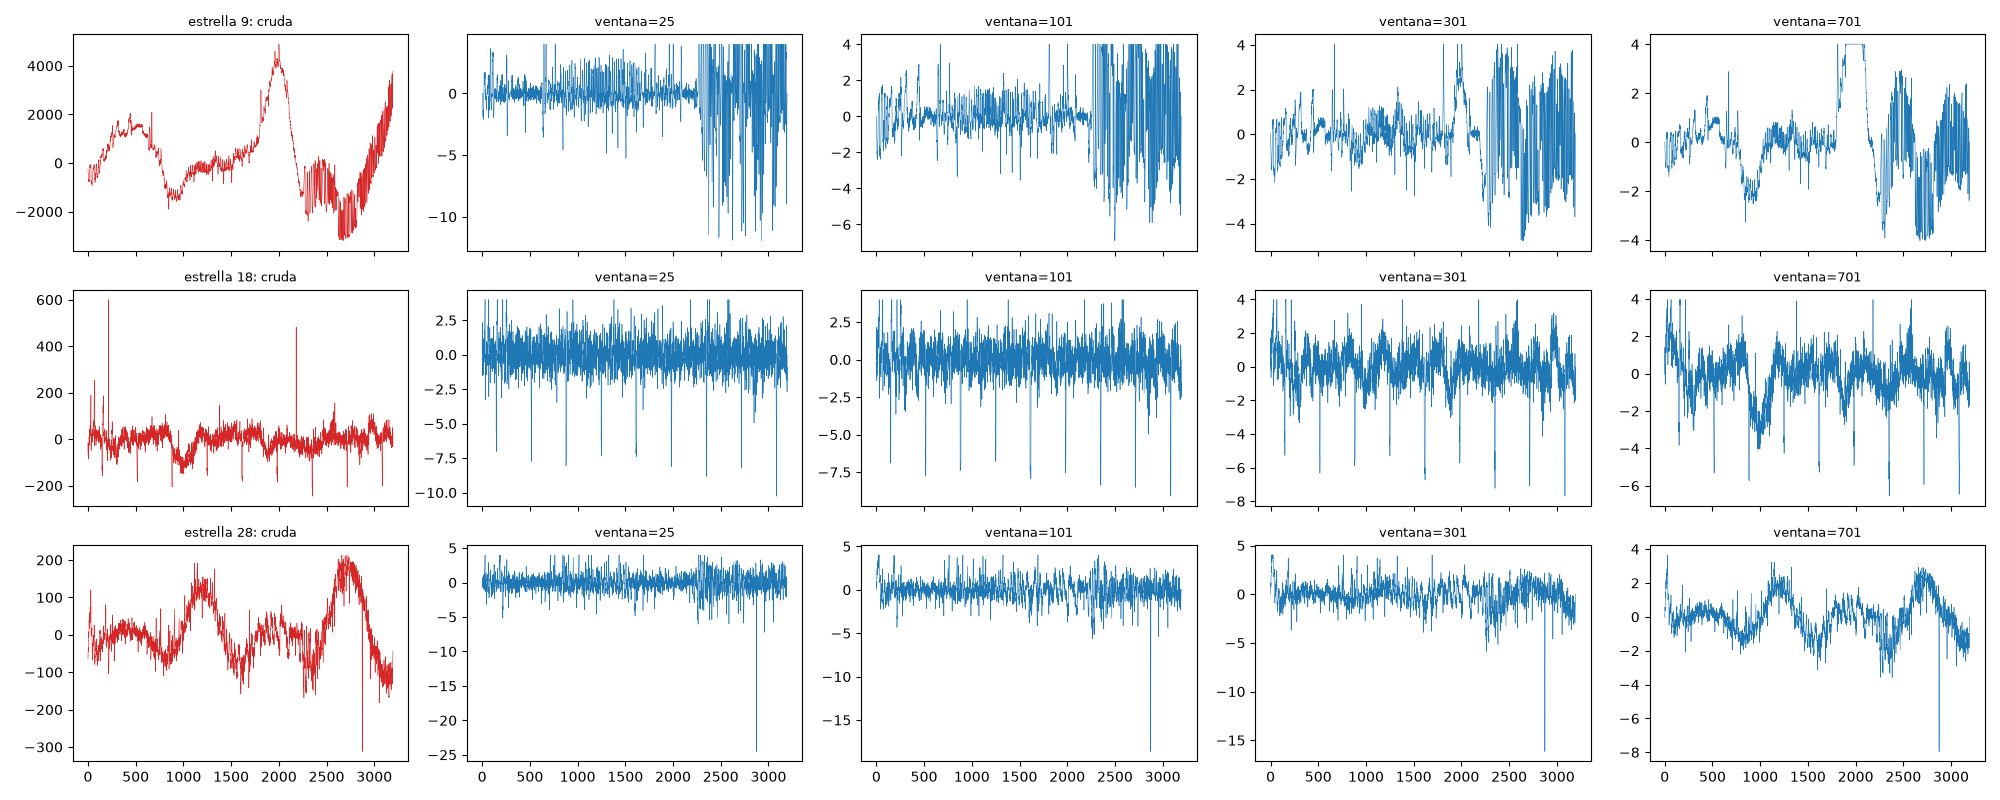
\includegraphics[width=\textwidth]{../../results/02_ventanas.png}
\caption{Tres estrellas con planeta: curva cruda (izquierda) y procesada con
ventanas de 25, 101, 301 y 701 puntos. En la estrella 18 las caídas periódicas
se ven con 25 y 101 y se pierden con 701.}
\label{fig:vent}
\end{figure}

% ------------------------------------------------------------------
\section{Primeros experimentos}

Todas las cifras son PR-AUC, cuyo valor al azar es 0{,}007 (la proporción de
positivos). Un modelo que siempre responde ``sin planeta'' obtiene 0{,}007 y una
regresión logística sobre 3 features simples $0{,}073\pm0{,}068$. La mejor
feature individual es el contraste del BLS (0{,}088).

\begin{table}[h]
\centering
\small
\begin{tabular}{@{}lcc@{}}
\toprule
\textbf{Features} & \textbf{Random Forest} & \textbf{XGBoost}\\
\midrule
Estadísticos (8) & $0{,}045\pm0{,}046$ & $0{,}030\pm0{,}018$\\
FFT (4) & $0{,}151\pm0{,}081$ & $0{,}129\pm0{,}076$\\
BLS (6) & $0{,}347\pm0{,}159$ & $0{,}305\pm0{,}161$\\
Todas (18) & $\mathbf{0{,}394\pm0{,}200}$ & $\mathbf{0{,}374\pm0{,}181}$\\
\bottomrule
\end{tabular}
\caption{PR-AUC (media $\pm$ desviación entre folds), CV 5$\times$5, según las
features usadas.}
\label{tab:abl}
\end{table}

\begin{table}[h]
\centering
\small
\begin{tabular}{@{}lccc|ccc@{}}
\toprule
& \multicolumn{3}{c|}{\textbf{CV 5 folds $\times$ 1}} & \multicolumn{3}{c}{\textbf{Test oficial (5 positivos)}}\\
\textbf{Modelo} & PR-AUC & Recall & Precisión & PR-AUC [IC 95\%] & Recall & Precisión\\
\midrule
CNN 1D & $0{,}27\pm0{,}16$ & 0{,}56 & 0{,}20 & 0{,}56 [0{,}37; 1{,}00] & 1{,}0 & 0{,}33\\
Random Forest & $0{,}42\pm0{,}18$ & 0{,}11 & 0{,}80 & 0{,}58 [0{,}16; 1{,}00] & 0{,}4 & 1{,}0\\
XGBoost & $0{,}37\pm0{,}18$ & 0{,}36 & 0{,}37 & 0{,}67 [0{,}29; 1{,}00] & 0{,}6 & 0{,}5\\
\bottomrule
\end{tabular}
\caption{CNN 1D frente a los modelos con las 18 features, sobre los mismos folds.
Recall y precisión con umbral 0{,}5, sin optimizar.}
\label{tab:cnn}
\end{table}

\textbf{Lectura.} (i)~Las features físicas importan: pasar de estadísticos a BLS
multiplica el PR-AUC por cerca de 8, y con todas se llega a unas 50 veces el
azar. (ii)~La FFT aporta poco: sumarla al BLS mejora de 0{,}35 a 0{,}39, menos
que la variación entre folds. (iii)~Random Forest y XGBoost rinden parecido.
(iv)~En CV la CNN rinde menos (0{,}27) pero es la que detecta más planetas
(recall 0{,}56, con más falsas alarmas); en el test ubica los 5 planetas entre
las posiciones 3 y 7 de 570. (v)~Con 5 positivos los intervalos casi se
solapan, así que no hay evidencia de que un modelo sea mejor; la CV (37
positivos) es la evidencia más confiable, y aun ahí la desviación entre folds
(${\sim}0{,}2$) supera muchas diferencias entre modelos.

% ------------------------------------------------------------------
\section{Riesgos y ajustes al plan}\label{sec:riesgos}

\begin{itemize}
  \item \textbf{Muy pocos positivos} (37 y 5): resultados inestables. Se
  mitiga con CV repetida e intervalos bootstrap, y el test oficial solo
  confirma.
  \item \textbf{Posible sesgo por campaña:} los positivos extra vienen de otras
  campañas y el modelo podría separar por origen y no por planeta. No lo hemos
  verificado; se revisará con saliencia, Grad-CAM y análisis de errores.
  \item \textbf{Supuesto de cadencia} de 30 minutos: afecta período y
  duración del BLS. Se medirá la sensibilidad variando la cadencia y el rango
  de períodos.
  \item \textbf{CNN por debajo del baseline:} hipótesis (sin probar): el
  \emph{global max pooling} detecta caídas pero no su repetición. Se probará
  \emph{data augmentation}, un entrenamiento más estable (menor peso de clase,
  tasa decreciente) y una variante que combine la CNN con features BLS.
  \item \textbf{Caída aislada interpretada como período:} en la estrella 28 el
  BLS usa una sola caída; se agregarán features de consistencia entre tránsitos.
  \item \textbf{Hiperparámetros y umbral sin ajustar:} se hará búsqueda con
  validación anidada y se elegirá el umbral en CV, no en el test.
  \item \textbf{Cómputo:} el BLS tarda unos 6 min en las 5.657 estrellas (12
  núcleos) y la CNN unos 7 min por 5 folds, por lo que una CV 5$\times$5
  de la CNN ($\approx$35 min) es viable.
\end{itemize}
\textbf{Calendario hasta el 20 de noviembre:} semana 1, \emph{augmentation} y
mejora de la CNN; semana 2, ablación completa y ajuste de hiperparámetros;
semana 3, interpretabilidad y sensibilidad a la cadencia; semana 4, informe
final, README y presentación.

% ------------------------------------------------------------------
\begingroup
\small
\bibliographystyle{plain}
\bibliography{refs}
\endgroup

\end{document}
